\section{Spiegeltraining en links/rechts-variatie}\label{app:mirror}
Deze proef onderbouwt de uitspraak over gespiegeld oefenen in de hoofdtekst. Alle 78.000 oorspronkelijke beelden en hun horizontale RGB-spiegelingen zijn afzonderlijk gedetecteerd: IMAGE-modus, maximaal twee handen, detectie- en aanwezigheidsdrempel 0,5. Er zijn 60.251 geldige originele detecties en 60.201 geldige spiegelingen. Handpunten en Left/Right-labels komen uit de eigen detectie van iedere presentatie; er worden geen anatomische puntindices verwisseld.

De SVM-referentie traint op geldige originele bronnen; de kandidaat voegt geldige spiegelingen van dezelfde trainingsbronnen toe. Elke bron behoudt totaalgewicht één. Imputatie, schaling, numerieke gamma en oorspronkelijke klassegewichten worden gedeeld. Bron en spiegeling blijven in dezelfde fold. Dit is een nieuwe detectieproef met een eigen referentie. De classificatiescores sluiten mislukte detecties uit, zoals bij de featurestudie.

Het vaste toetsmengsel selecteert met seed 20261106 per letter/fold de helft van de bronnen voor spiegeling: 39.000 originele en 39.000 gespiegelde beelden. Selectie is onafhankelijk van detectiesucces. Na uitsluiting van mislukte detecties blijven 60.225 beelden over. Binnen elke presentatie krijgen beide modellen exact dezelfde geaccepteerde toetsbeelden. Het mengsel is een andere toetsverdeling dan uitsluitend oorspronkelijke foto's.

\begin{table}[h]\centering\small
\caption{SVM-classificatie bij geldige handdetectie; mislukte detecties zijn uitgesloten. N geldig is de noemer per presentatie; P is macro-precisie. Alle-pogingenscores, inclusief detectiemislukkingen, blijven beschikbaar in de resultaatbestanden.}
\begin{tabular}{llrrrr}\toprule
Toetsbeelden & Training & N geldig & P (\%) & Macro-F1 & Correct\\\midrule
\tableinput appendix_mirror_nl.tex
\bottomrule\end{tabular}\end{table}

Op het mengsel zijn er netto 22.349 extra correcte pogingen. Op uitsluitend oorspronkelijke beelden zijn het er 26 minder. De winst betreft dus een specifieke synthetische presentatieverdeling. Spiegelparen delen persoon, pose en achtergrond; zij zijn geen onafhankelijke linkshandige deelnemers. Left/Right is bovendien een detectoruitvoer, geen geverifieerd menselijk label.

\clearpage
\subsection{Geselecteerde spiegelbeelden}
De volgende voorbeelden tonen de oorspronkelijke foto en de apart gedetecteerde spiegeling. Dezelfde bron komt bij het voorspellen niet in de training van de betreffende fold voor.
\begin{figure}[h]\centering
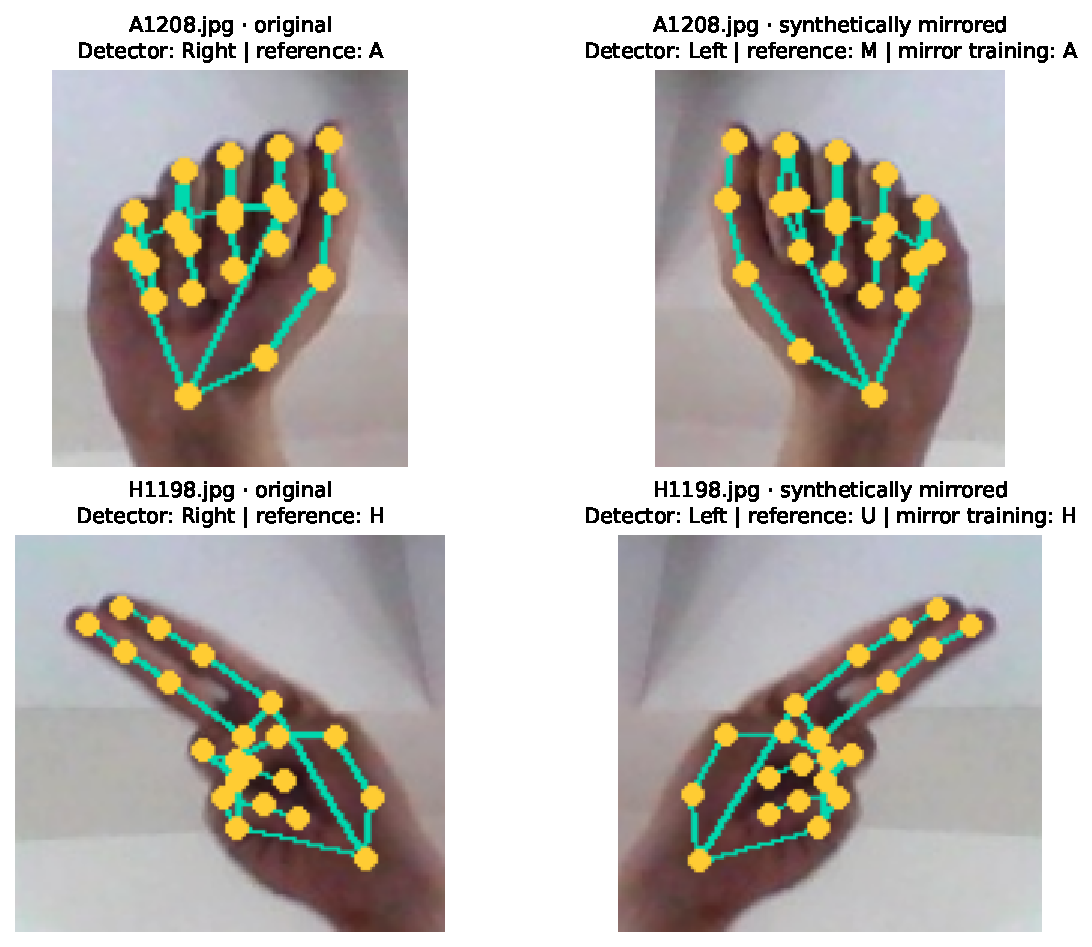
\includegraphics[width=.86\linewidth]{figures/mirror_examples.pdf}
\caption{Geselecteerde voorbeelden A1208 en H1198: origineel links, synthetische spiegeling rechts. Zonder spiegeltraining worden de spiegelingen M en U genoemd; met spiegeltraining A en H. De voorspellingen komen uit fold 5, waarin deze bronnen niet voor training zijn gebruikt. De figuur illustreert een bestaand resultaat, geen nieuwe onafhankelijke test.}
\end{figure}

Per A/H is het eerste passende bron-ID gekozen met een geldige Right/Left-detectie, een correcte oorspronkelijke voorspelling, een fout spiegelbeeld zonder spiegeltraining en herstel daarmee. Deze selectie schat geen succespercentage. Spiegelen maakt een zichtbare handpalm geen handrug. Alle voorspellingen, detectie- en modelinstellingen staan in \texttt{results/mirror\_01/}; de beeldselectie en hashes in \texttt{results/appendix\_visuals\_01/}.
